\section{Results}\label{sec:results}


\subsection{Lognormal Mocks}

Corner plots of the PNG parameter $\fnl$ and bias coefficient are shown in Fig. \ref{fig:mcmc_mocks} for fitting the mean power spectrum of the mocks, with and without $\fnl$. Maximum-A-Posteriori estimates and marginalized mean, median and $1\sigma$ quantiles are summarized in Tab. \ref{tab:mocksmcmc}. As a robustness test, we also fit the mean power spectrum of the $\fnl=100$ mocks using the covariance matrix estimated from the $\fnl=0$ mocks. We find that the constraints improve by a factor of $4.2$, due to a higher signal to noise ratio.
\begin{figure}
    \centering
    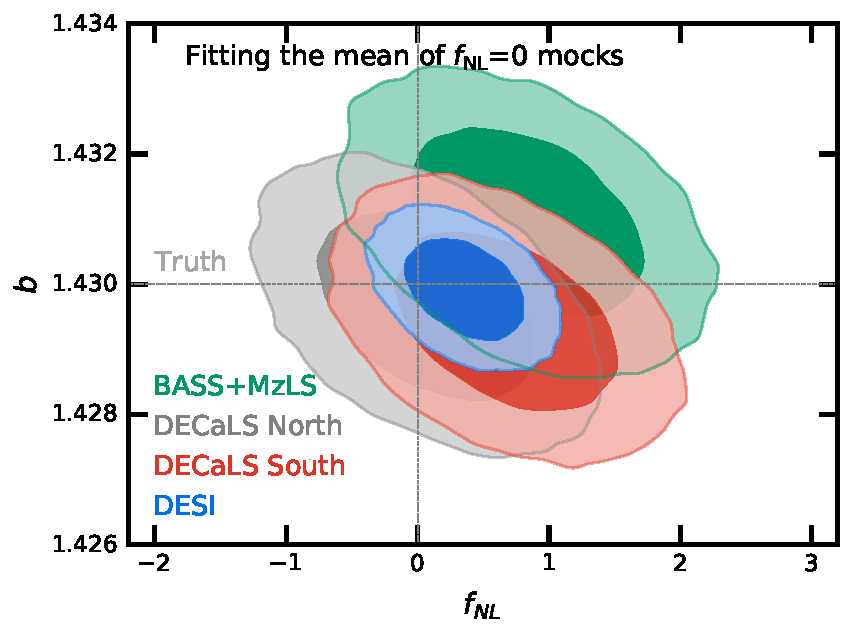
\includegraphics[width=0.45\textwidth]{figures/mcmc_zero.pdf} 
    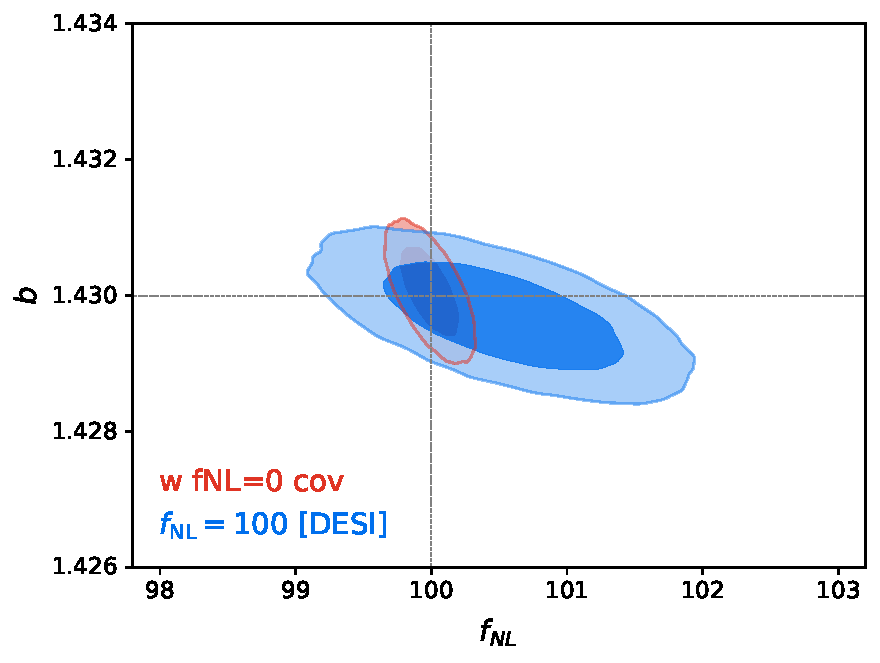
\includegraphics[width=0.45\textwidth]{figures/mcmc_po100.pdf} 
    \caption{Lognormal mocks for $\fnl=0$ and $100$.}\label{fig:mcmc_mocks}
\end{figure}


\begin{table*}
  \begin{center}
    \caption{Best fit Maximum-A-Posteriori (MAP) and marginalized stats for $\fnl$ from fitting the mean power spectrum of the mocks.}
    \label{tab:mocksmcmc}
    \begin{tabular}{lcccccc}
    \hline
    \hline
   $\fnl$ [footprint] & MAP [scipy] & MAP [chain]  &	Mean [chain]	& Median [chain] &	16th	& 84th \\
    \hline
	0~~~[BASS+MzLS]	&0.757876&	0.764393&	0.753563&	0.764325&	-0.009674&	1.519141 \\
	0~~~[DECaLS North]	&0.177116&	0.178279&	0.154977&	0.159582&	-0.543994&	0.857133\\
	0~~~[DECaLS South]&	0.650587&	0.654956&	0.632435&	0.635791&	0.084512&	1.178858 \\
	0~~~[DESI] & 0.572941	& 0.569411 &	0.563005&	0.564670&	0.203400&	0.921198 \\
	100~[DESI] & 100.530435	& 100.528862 &	100.526471&	100.528808&	99.952158&	101.100725 
    \end{tabular}
  \end{center}
\end{table*}


\clearpage
\subsection{DR9 LRGs}
\begin{figure*}
    \centering
    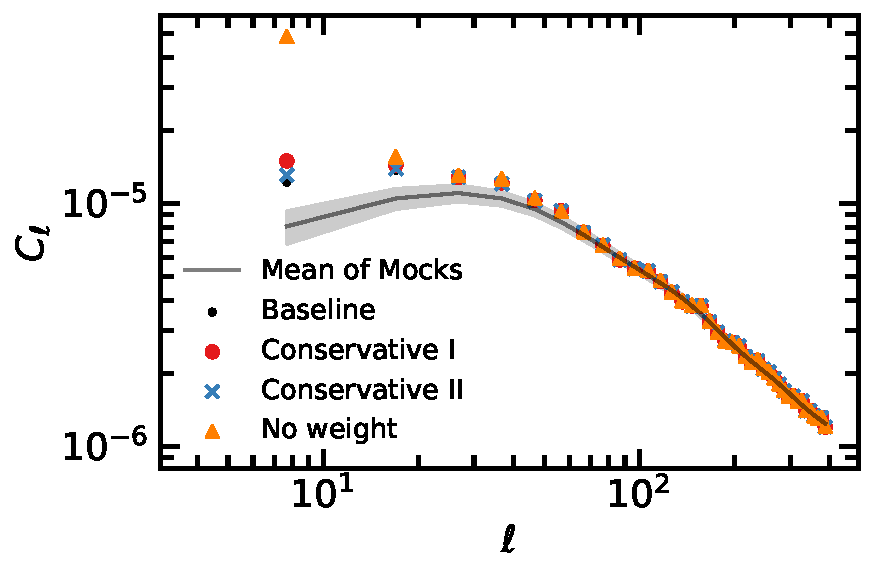
\includegraphics[width=0.95\textwidth]{figures/cl_obs.pdf} 
    \caption{Measured power spectrum of the DR9 LRG sample before and after correcting for systematics with their corresponding best fit theory predictions. The shade represents $1\sigma$ error on the mean power spectrum of mocks.}
    \label{fig:cl_dr9}
\end{figure*}

\begin{figure*}
    \centering
    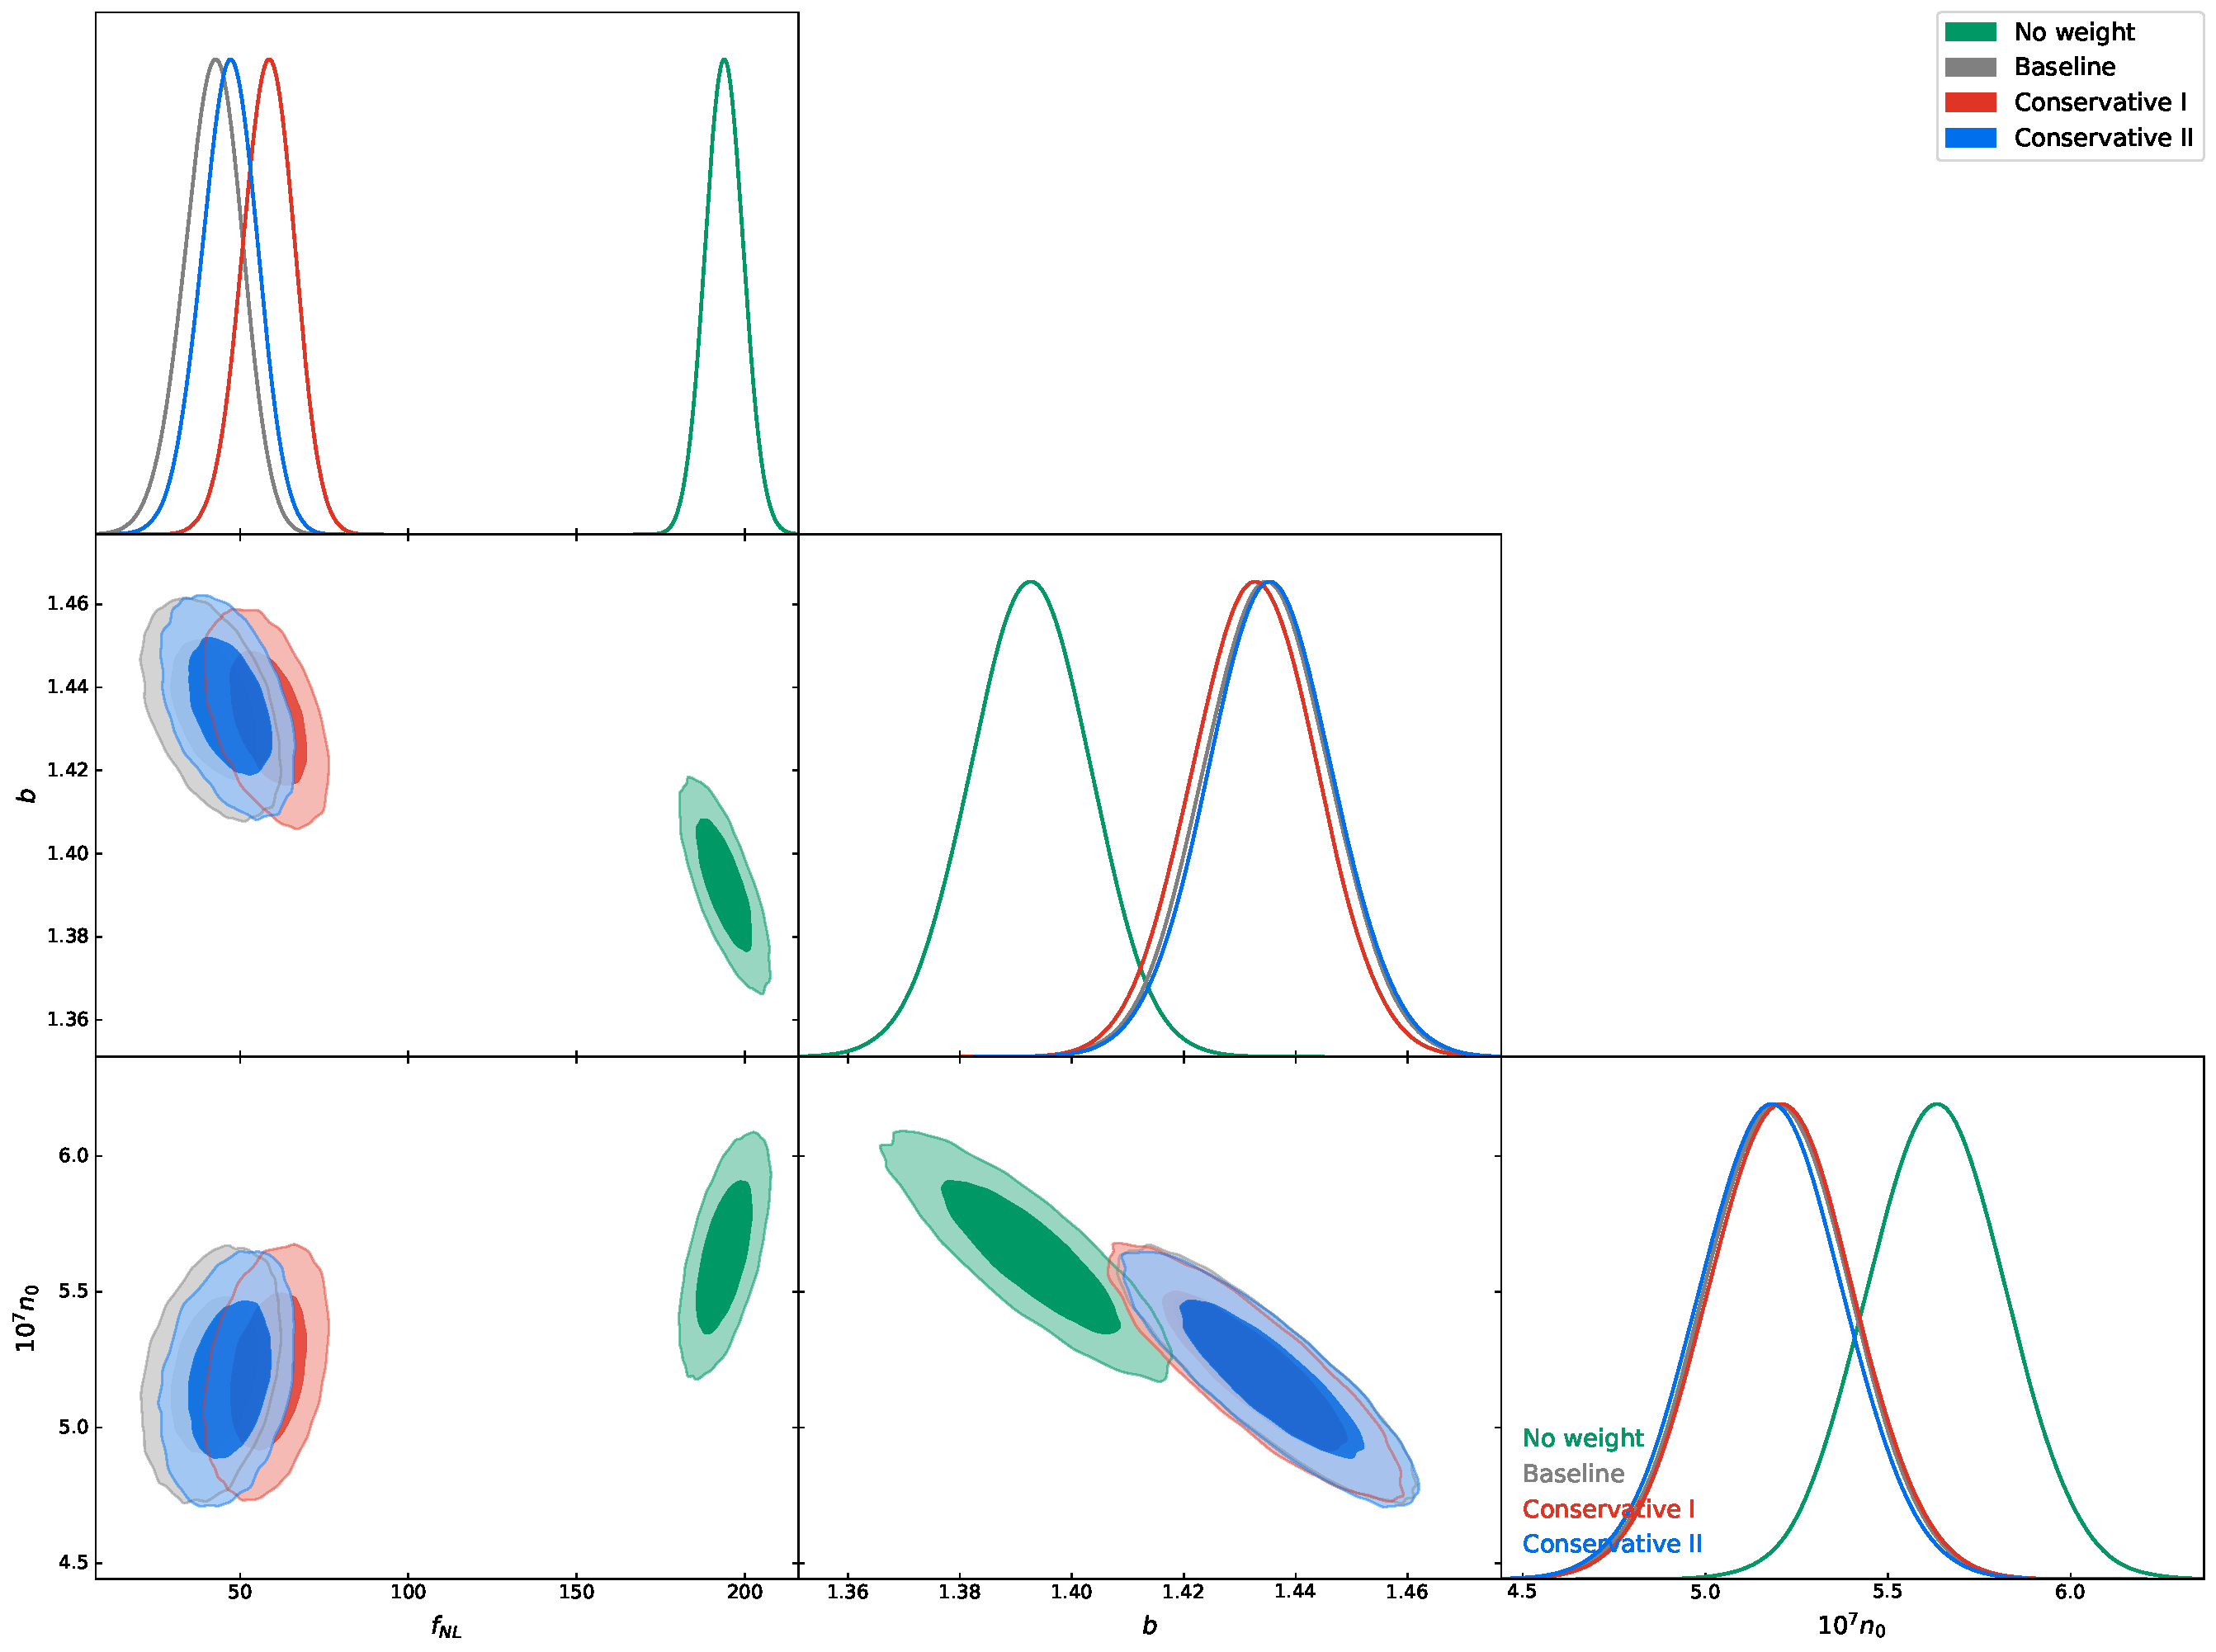
\includegraphics[width=0.95\textwidth]{figures/mcmc_dr9.pdf} 
    \caption{DR9 LRGs for DESI footprint.}\label{fig:mcmc_dr9}
\end{figure*}

\begin{figure*}
    \centering
    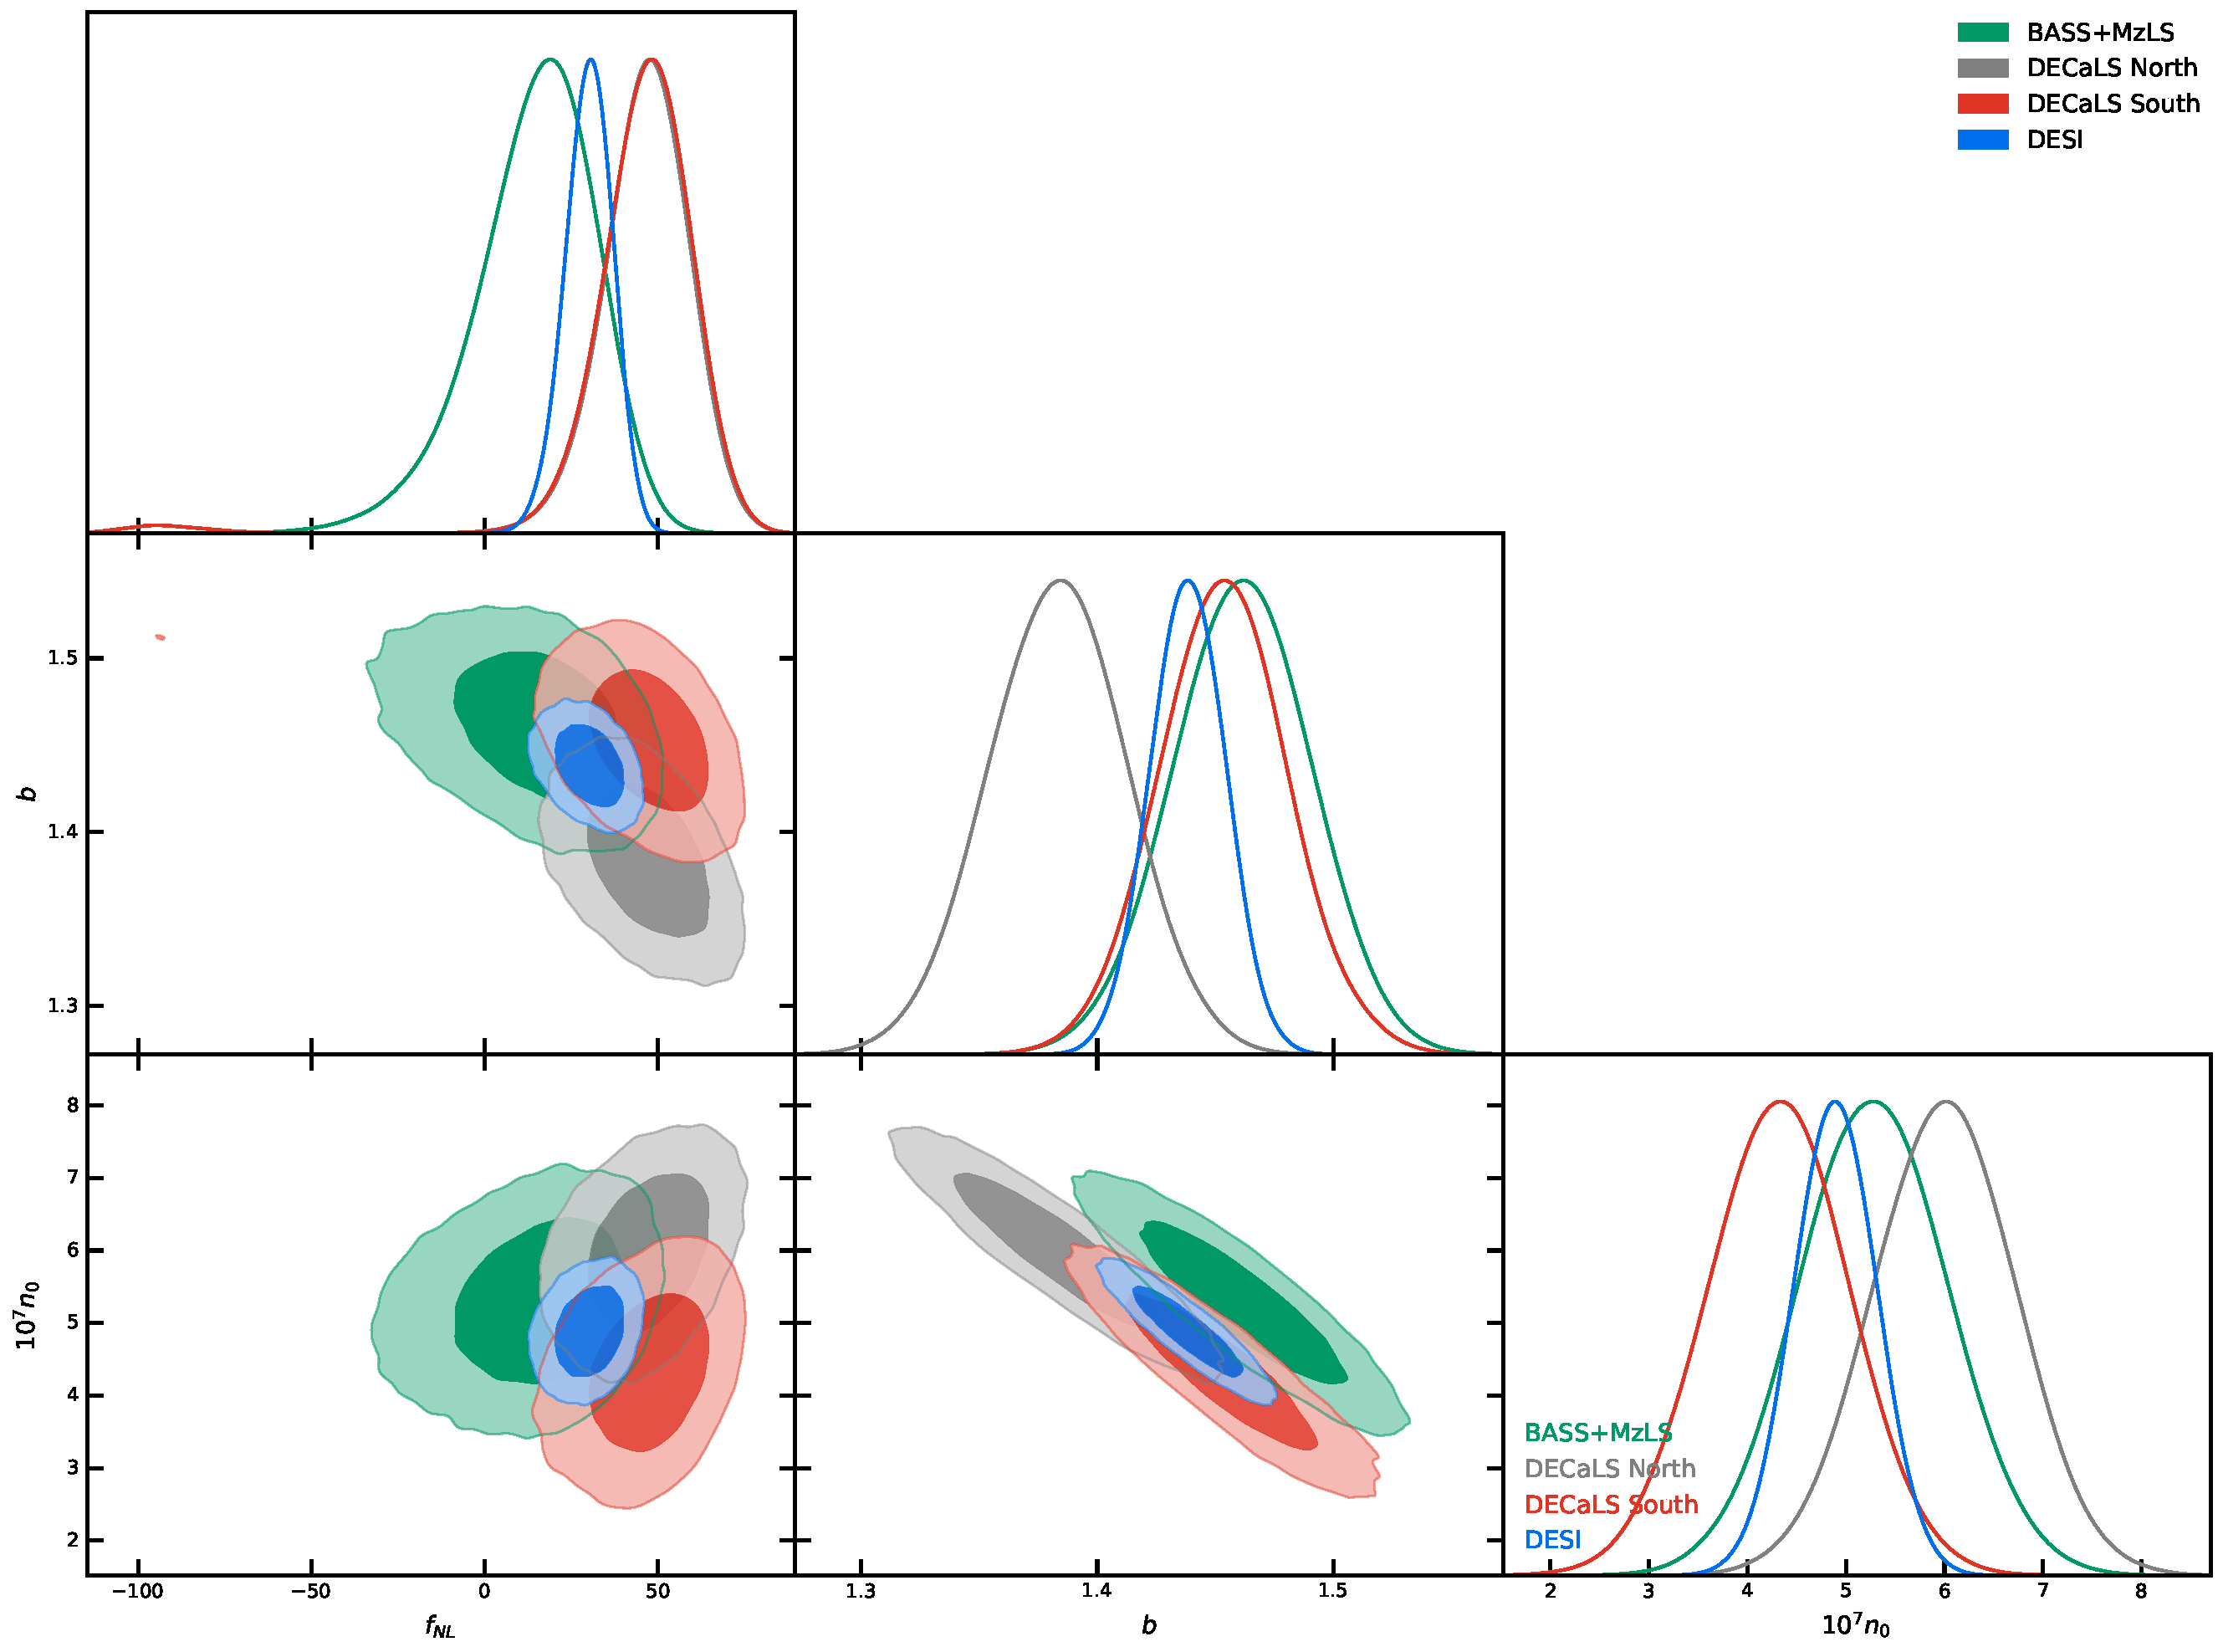
\includegraphics[width=0.95\textwidth]{figures/mcmc_dr9_2.pdf} 
    \caption{DR9 LRGs for each individual imaging survey.}\label{fig:mcmc_dr9_2}
\end{figure*}

\begin{table*}
  \begin{center}
    \caption{Best fit Maximum-A-Posteriori (MAP) and marginalized stats for $\fnl$ from fitting power spectrum of DR9 LRGs for DESI footprint before and after correcting for systematics.}
    \label{tab:dr9mcmc}
    \begin{tabular}{lcccccc}
    \hline
    \hline
    & MAP [scipy] & MAP [chain]  &	Mean [chain]	& Median [chain] &	16th	& 84th \\
    \hline
No Weight&	248.473520	&248.411797	&248.776187	&248.595088&	242.599638&	254.977561\\
Baseline	&53.373443	&53.302632	&53.045753	&53.111457	&47.514519	&58.661667\\
Conservative I	&65.286775	&65.277211	&65.047508&	65.122821&	60.079103&	70.028714\\
Conservative II	&57.480562	&57.384026	&57.308910&	57.401921&	51.999420&	62.589189\\
Nonlinear (Cons. II)	&42.845528	&42.682128	&42.255626&	42.360824&	36.203137&	48.370399 \\
Nonlinear (Depths+EBV)	&51.662924 &	51.553357&	51.246052&	51.351139	 & 45.627949&	56.829878

    \end{tabular}
  \end{center}
\end{table*}


\begin{table*}
  \begin{center}
    \caption{Best fit Maximum-A-Posteriori (MAP) and marginalized stats for $\fnl$ from fitting power spectrum of DR9 LRGs  for different footprints after the nonlinear treatment with Conservative II.}
    \label{tab:dr9mcmc}
    \begin{tabular}{lcccccc}
    \hline
    \hline
    & MAP [scipy] & MAP [chain]  &	Mean [chain]	& Median [chain] &	16th	& 84th \\
    \hline
BASS+MzLS&	21.249515&	21.157945&	14.725741&	17.215942&	-3.156691&	33.469937\\
DECaLS North&	56.795210&	56.936222&	55.269142&	55.809133&	43.477820&	67.443802\\
DECaLS South &	51.334244&	51.166450&	50.637556&	50.878139&	42.450484&	58.794574
    \end{tabular}
  \end{center}
\end{table*}




%
%fNL = 100	100.853749	100.857356	100.856818	100.857763	100.306626	101.406558
